% Begin section ----------------------------------------------------------------
\section{Question 1}

% Part (a) ---------------------------------------------------------------------
\begin{frame}{Part (a)}

    We have that:
    \begin{align*}
        Y = -X^2 + (2 + \varepsilon) X
    \end{align*}
    
    The effect of a marginal change of $X$ in $Y$ is simply:
    \begin{align*}
        \frac{\partial Y}{\partial X} = -2 X + (2 + \varepsilon)
    \end{align*}

    These effects are heterogeneous. Farms with good soil will have $\varepsilon = 1$, and so the marginal effect is $-2 X + 3$. Farms with bad soil have $\varepsilon = -1$ and so the marginal effect is $- 2X + 1$.
\end{frame}

% Part (b) ---------------------------------------------------------------------
\begin{frame}{Part (b)}

    To find the $ACE$ of $X$ on $Y$ as a function of $X$ we have to integrate out $\varepsilon$. This can be done in two steps. First, find the marginal density of $X$:
    \begin{align*}
        f_X(x) &= \int_{-1}^1 f_{X \varepsilon}(x, z) d z
        \\
        &= \int_{-1}^1 \frac{1 + x - z}{8} dz
        \\
        &= \varepsilon \Biggr( \frac{1 + x}{8} \Biggr) - \frac{z^2}{16} \Biggr |_{z=-1}^{z=1}
        \\
        &= \frac{1 + x}{4}
    \end{align*}

\end{frame}

\begin{frame}{Part (b)}

    Now that we have the marginal density of $X$, we can calculate the conditional density:
    \begin{align*}
        f_{\varepsilon \mid X}(z \mid x) &= \frac{f_{X \varepsilon} (x, z) }{f_X (x)}
        \\
        &= \frac{1 + x - z}{2 + 2x}
    \end{align*}

    Finally, the $ACE$ is then:
    \begin{align*}
        ACE(X) &= \int_{-1}^1 (- 2 x + 2 + z) \Biggr( \frac{1 + x - z}{2 + 2x} \Biggr) dz
        \\
        &= \frac{5 - 6X^2}{3X + 3}
    \end{align*}

\end{frame}

\begin{frame}{Part (b)}

    \begin{figure}[ht]
        \centering
        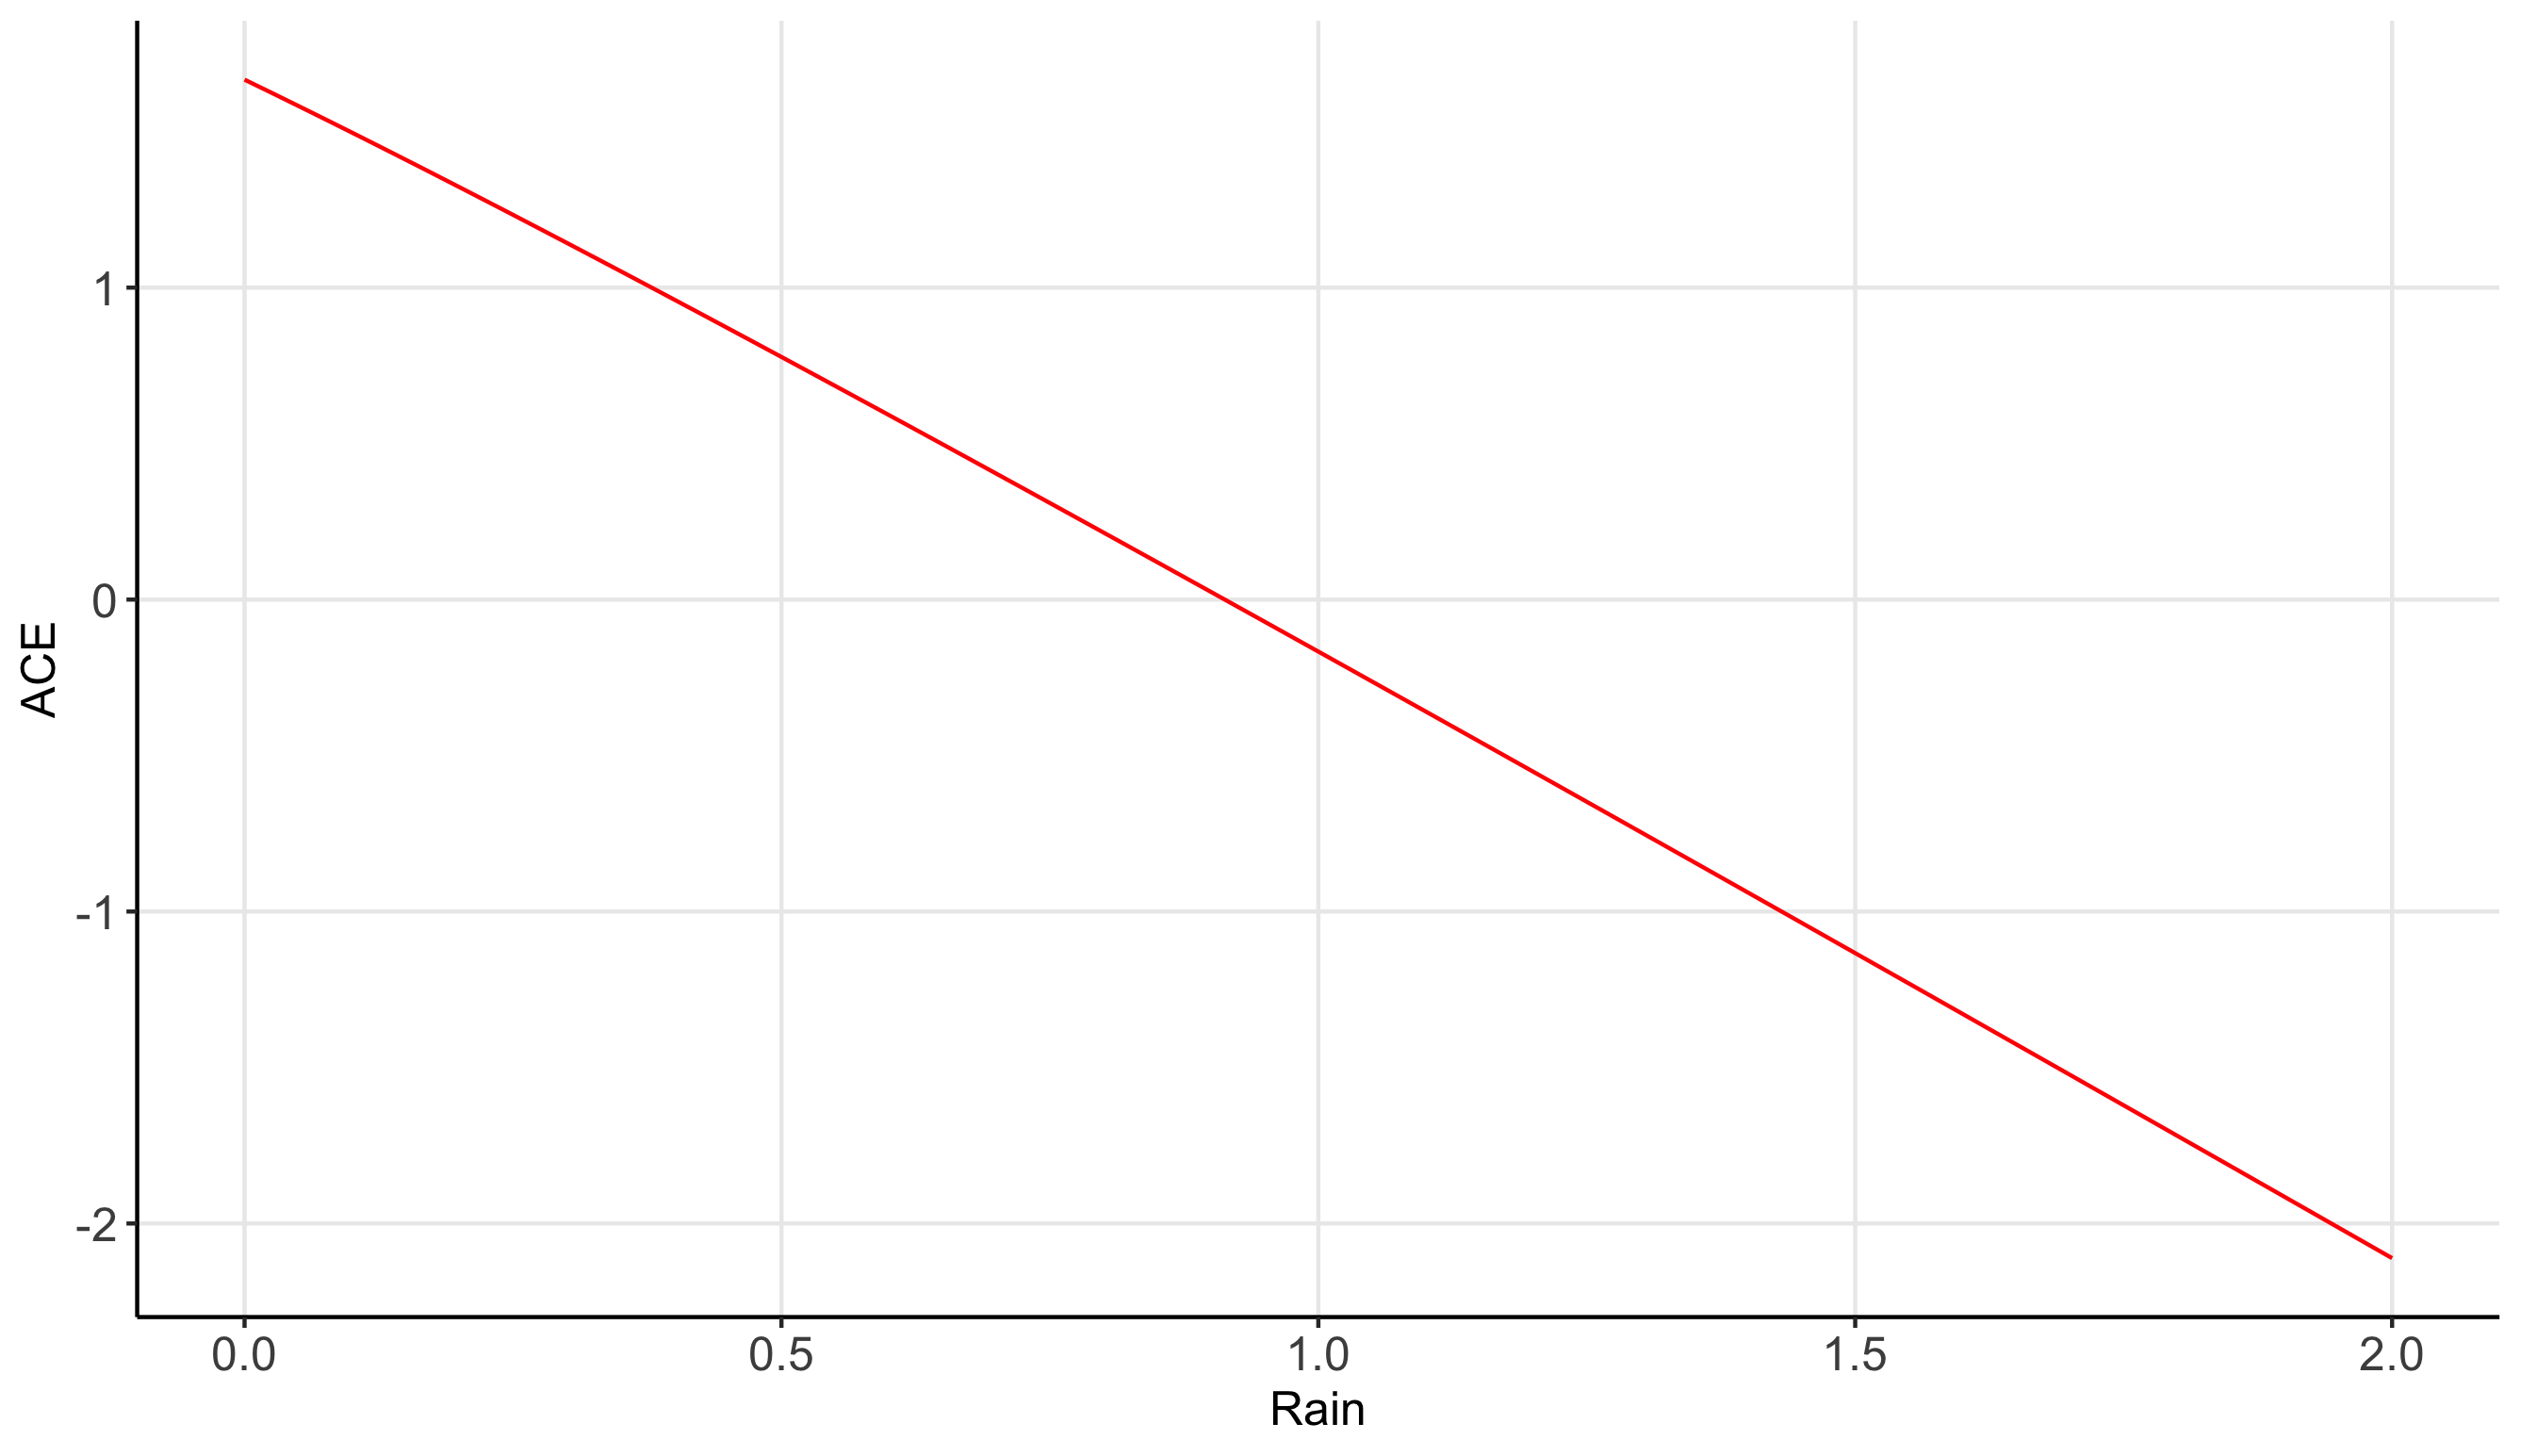
\includegraphics[width=1.0\linewidth]{./resources/question-1-b.png}
    \end{figure}

\end{frame}

% Part (c) ---------------------------------------------------------------------
\begin{frame}{Part (c)}

    To find the unconditional expectation just proceed as usual for a continuous variable:
    \begin{align*}
        \mathbb{E}[Y] &= \mathbb{E}[-X^2 + (2 + \varepsilon) X]
        \\
        &= \int_0^2 \int_{-1}^1 (-x^2 + (2 + z) x) f_{X \varepsilon}(x, z) dz dx
        \\
        &= \int_0^2 \int_{-1}^1 (-x^2 + (2 + z) x) \frac{1 + x - z}{8} dz dx
        \\
        &= \frac{1}{2}
    \end{align*}

\end{frame}

\begin{frame}{Part (c)}

    And the conditional mean:
    \begin{align*}
        \mathbb{E}[Y \mid X] &= \mathbb{E}[-X^2 + (2 + \varepsilon) X \mid X]
        \\
        &= -X^2 + X \mathbb{E}[ (2 + \varepsilon) \mid X]
        \\
        &= -X^2 + X \int_{-1}^1 (2 + z) f_{\varepsilon \mid X}(z \mid x) dz
        \\
        &= -X^2 + X \int_{-1}^1 (2 + z) \Biggr( \frac{1 + X - z}{2 + 2X} \Biggr) dz
        \\
        &= -X^2 + X \frac{6X  + 5}{3X + 3}
    \end{align*}

\end{frame}

\begin{frame}{Part (c)}

    In case you were skeptical about the Law of Iterated Expectations:
    \begin{align*}
        \mathbb{E}[Y] &= \mathbb{E}[ \mathbb{E}[Y \mid X] ]
        \\
        &= \int_0^2 f_X(x) \mathbb{E}[Y \mid X] dx
        \\
        &= \int_0^2 \Biggr( \frac{1+x}{4} \Biggr) \Biggr( -X^2 + X \frac{6X  + 5}{3X + 3} \Biggr) dx
        \\
        &= \frac{1}{2}
    \end{align*}

\end{frame}

% Part (d) ---------------------------------------------------------------------
\begin{frame}{Part (d)}

    Note that
    \begin{align*}
        \frac{\partial}{\partial X} \mathbb{E}[Y \mid X] = -2X + \frac{6X^2 + 12X + 5}{3(X + 1)^2} > \frac{5 - 6x^2}{3(x + 1)} = ACE(X)
    \end{align*}

    We can see that:
    \begin{align*}
        \frac{\partial}{\partial X} \mathbb{E}[Y \mid X] - ACE(X) &= -2X + \frac{6X^2 + 12X + 5}{3(X + 1)^2} - \frac{5 - 6x^2}{3(x + 1)}
        \\
        &= \frac{X}{3(x + 1)^2} > 0
    \end{align*}

    This means that the slope of the regression overstates the causal effect of rain $X$. Why does this happen? What is the CEF capturing?

\end{frame}

% Part (e) ---------------------------------------------------------------------
\begin{frame}{Part (e)}

    Let's do this by parts. We can calculate the variance of $X$ as:
    \begin{align*}
        \operatorname{Var}(X) &= \mathbb{E}[X^2] - \mathbb{E}[X]^2
        \\
        &= \int_0^2 x^2 f_X(x) dx - \Biggr( \int_0^2 x f_X(x) dx \Biggr)^2
        \\
        &= \int_0^2 x^2 \Biggr( \frac{1+x}{4} \Biggr) dx - \Biggr( \int_0^2 x \Biggr( \frac{1+x}{4} \Biggr) dx \Biggr)^2
        \\
        &= \frac{5}{3} - \Biggr( \frac{7}{6} \Biggr)^2
        \\
        &= \frac{11}{36}
    \end{align*}

\end{frame}

\begin{frame}{Part (e)}

    And the co-variance of $X$ and $Y$ is:
    \begin{align*}
        \operatorname{Cov}(X, Y) &= \mathbb{E}[XY] - \mathbb{E}[X] \mathbb{E}[Y]
        \\
        &= \mathbb{E}[X^2(- X + 2 + \varepsilon)] - \mathbb{E}[X] \mathbb{E}[Y]
        \\
        &= \int_0^2 \int_{-1}^1 x^2(- x + 2 + z) f_{X \varepsilon} (x, z) d z dx - \mathbb{E}[X] \mathbb{E}[Y]
        \\
        &= \int_0^2 \int_{-1}^1 x^2(- x + 2 + z) \Biggr( \frac{1 + x - z}{8} \Biggr) d z dx - \frac{7}{12}
        \\
        &= \frac{23}{45} - \frac{7}{12}
        \\
        &= -\frac{13}{180}
    \end{align*}

\end{frame}

\begin{frame}{Part (e)}

    Recall that the BLP of $Y$ given $X$ is $Y = \beta_0 + \beta_1 X$ where:
    \begin{align*}
        \beta_1 &= \frac{\operatorname{Cov}(X, Y)}{\operatorname{Var}(X)} = -\frac{13}{55}
        \\
        \beta_0 &= \mathbb{E}[Y] - \beta_1 \mathbb{E}[X] = \frac{128}{165}
    \end{align*}

    So we have:
    \begin{align*}
        BLP(Y \mid X) = \frac{128}{165} - \frac{13}{55} X
    \end{align*}
    
    If this is true and causal, an increase in rain $X$ will increase production $Y$ by $-\frac{13}{55}$

\end{frame}